\documentclass[fleqn,10pt,doc,onecolumn]{SelfArx}%article} % Document font size and equations flushed left

\usepackage{float}
\usepackage{graphicx}
\usepackage{caption}
\usepackage[hyphens]{url}
\usepackage{hyperref}
\usepackage{xcolor}
\usepackage{amsmath}
\graphicspath{{figures/}}
\setlength{\abovecaptionskip}{15pt plus 3pt minus 2pt}

\newcommand{\beginsupplement}{%
        \setcounter{table}{0}
        \renewcommand{\thetable}{S\arabic{table}}%
        \setcounter{figure}{0}
        \renewcommand{\thefigure}{S\arabic{figure}}%
     }

\definecolor{color1}{RGB}{0,0,90} % Color of the article title and sections
\definecolor{color2}{RGB}{200,200,200} % Color of the boxes behind the abstract and headings
\definecolor{color3}{RGB}{5,5,5} % Color of the boxes behind the abstract and headings

\JournalInfo{.} % Journal information ``Journal, Vol. XXI, No. 1, 1-5, 2015''
\Archive{ } % Additional notes (e.g. copyright, DOI, review/research article)

\PaperTitle{A Bioinformatician, Computer Scientist, and Geneticist lead bioinformatic tool development - which one is better?} % Article
                                                                                                                               % title

\Authors{Paul P. Gardner\textsuperscript{1}*}
  
\affiliation{\textsuperscript{1}\textit{Department of Biochemistry, University of Otago, Dunedin, New Zealand.}} % Author affiliation
\affiliation{*\textbf{Corresponding author}: paul.gardner@otago.ac.nz} % Corresponding author


\Keywords{} % Keywords - if you don't want any simply remove all the text between the curly brackets
\newcommand{\keywordname}{Keywords} % Defines the keywords heading name

%----------------------------------------------------------------------------------------
%       ABSTRACT
%----------------------------------------------------------------------------------------


% The abstract could benefit from a clearer statement of the research question, methodology, and key findings. It currently mixes multiple ideas without a clear flow.
\Abstract{The development of accurate bioinformatic software tools is
  critical for the effective analysis of complex biological data. This
  study investigates the relationship between the academic department
  affiliations of authors and the accuracy of the bioinformatic tools
  they develop. By analyzing a corpus of previously benchmarked
  bioinformatic software tools, we mapped tools to academic fields of
  corresponding authors and evaluated tool accuracy by field. Our
  results indicate that "Medical Informatics," categorized under
  "Technologies," outperforms other fields in terms of software
  accuracy, with a mean proportion of wins in accuracy rankings higher
  than the null expectation. Conversely, tools developed by authors
  affiliated with "Bioinformatics" and "Engineering" fields produce
  lower accuracy tools. After correcting for multiple testing, no
  result is significant ($p>0.05$). Our findings show a distinct lack
  of an association between academic field and bioinformatic software
  accuracy, highlighting that the development of interdisciplinary
  software applications can be hosted by any aligned department with
  sufficient resources.  }


\begin{document}

\flushbottom % Makes all text pages the same height
\maketitle % Print the title and abstract box
%\tableofcontents % Print the contents section

\thispagestyle{empty} % Removes page numbering from the first page


\section*{Background}

% The introduction lacks a strong hook or clear statement of the problem being addressed. It would be helpful to more explicitly state the importance of understanding the relationship between academic department affiliation and bioinformatics tool accuracy.

Much is made of departmental divisions within academia; These can
denote research and teaching expertise \cite{ben2016s}, influence
hiring decisions, access to funding, publishing and the training of
students recruited for research projects
\cite{bourke1998institutions}. However, interdisciplinary subjects
such as bioinformatics break down the traditional barriers between
departments and subject areas
\cite{Ouzounis:2003,Eddy:2005,hogeweg2011roots}.

Bioinformatics, is an interdisciplinary field that fuses biology,
computer science, and mathematics, and now plays a pivotal role in
modern biological research \cite{Ouzounis:2003}. The development of
bioinformatic tools and software is critical for interpreting complex
biological questions, such as what evolutionary, structural and
functional analyses of genomic, transcriptomic, and proteomic data can
tell us. The field of ``bioinformatics'' can include many overlapping
research fields that include computational biology, biomathematics,
biostatistics, medical informatics and other similar areas.

Bioinformatics began gaining traction with the advent of
high-throughput sequencing technologies, necessitating robust
computational tools to handle the large amounts of data generated
\cite{Ouzounis:2003,hogeweg2011roots}. Departments specializing in
bioinformatics emerged from biology, computer science, and engineering
faculties, each contributing to the field's growth.

Bioinformatics inherently requires a multidisciplinary
approach. Interdisciplinary research allows for the integration of
methods and perspectives from different disciplines, leading to novel
insights and solutions that a single discipline might not achieve
independently \cite{mazzocchi2019scientific}.  This is especially
relevant in bioinformatics, where expertise in biological sciences is
crucial for understanding the data, while computational skills are
needed to develop and implement algorithms, and analyze and interpret
data.

The \textbf{biological and health sciences,} in particular genetics,
biochemistry and molecular biology provide essential domain knowledge,
ensuring that the software tools developed are biologically relevant
and accurate.  Biologists can identify the critical biological
questions and ensure that the computational tools are designed to
address these questions effectively. However, biology departments may
lack the advanced computational expertise required for sophisticated
software development. We have grouped the biological and health fields
into ``\textbf{domain experts}'' in the following analysis.

The \textbf{mathematical, engineering and computational sciences}, or
the ``\textbf{development experts}'' as we have dubbed them here,
contribute significantly by providing expertise in algorithm
development, data structures, and software engineering
principles. These skills are essential for creating efficient,
scalable, and robust bioinformatic tools. Nonetheless, the challenge
for computer science, engineering and mathematics or statistics
departments lies in acquiring a deep understanding of biological
domains necessary to ensure the relevance and accuracy of their
software tools.

Departmental differences might matter in the development of
bioinformatic software tools as they can reflect the the varying
expertise, resources, and perspectives that different academic fields
bring to the table. The development experts may excel in algorithm
efficiency, mathematical modelling, data handling and software engineering. However,
the domain experts may bring a deep understanding of biological
questions, data interpretation and limitations, and possibly better
curation of control datasets. As a result, the success of a tool may
depend more on the integration of diverse expertise rather than the
specific departmental affiliation of its developers. This blending of
skills could neutralize any potential disparities between departments,
leading to comparable outcomes regardless of the department of origin.

As the field of bioinformatics evolves, and the dependence on research
software tools increases due to growing data volumes, this study seeks
to determine whether the academic department of a corresponding author
is associated with the accuracy of the bioinformatic software tools
they develop. Specifically, we investigate whether the presumed
subject expertise, as indicated by the author's departmental
affiliation, has a measurable impact on the accuracy of these tools,
using a benchmarked corpus of bioinformatic software tools to assess
this relationship.

%% \textbf{Engineering}, particularly those focusing on
%% bioengineering and systems biology, bridge the gap between biological
%% sciences and computational techniques. They often have a strong
%% emphasis on interdisciplinary research, which is vital for
%% bioinformatics. These departments can leverage their strengths in both
%% domains to develop integrated solutions.

%% Nick Loman and Mick Watson (2013) argue that a good computational
%% biologist must understand both the biological questions and the
%% computational methods used to address them (Loman \& Watson
%% nbt.2740). This dual expertise is often best nurtured in departments
%% that prioritize interdisciplinary training and collaboration.


%% \textbf{The developer expert, domain expert or interdisciplinary scientist ...}


\begin{figure*}[ht!]
\begin{center}
  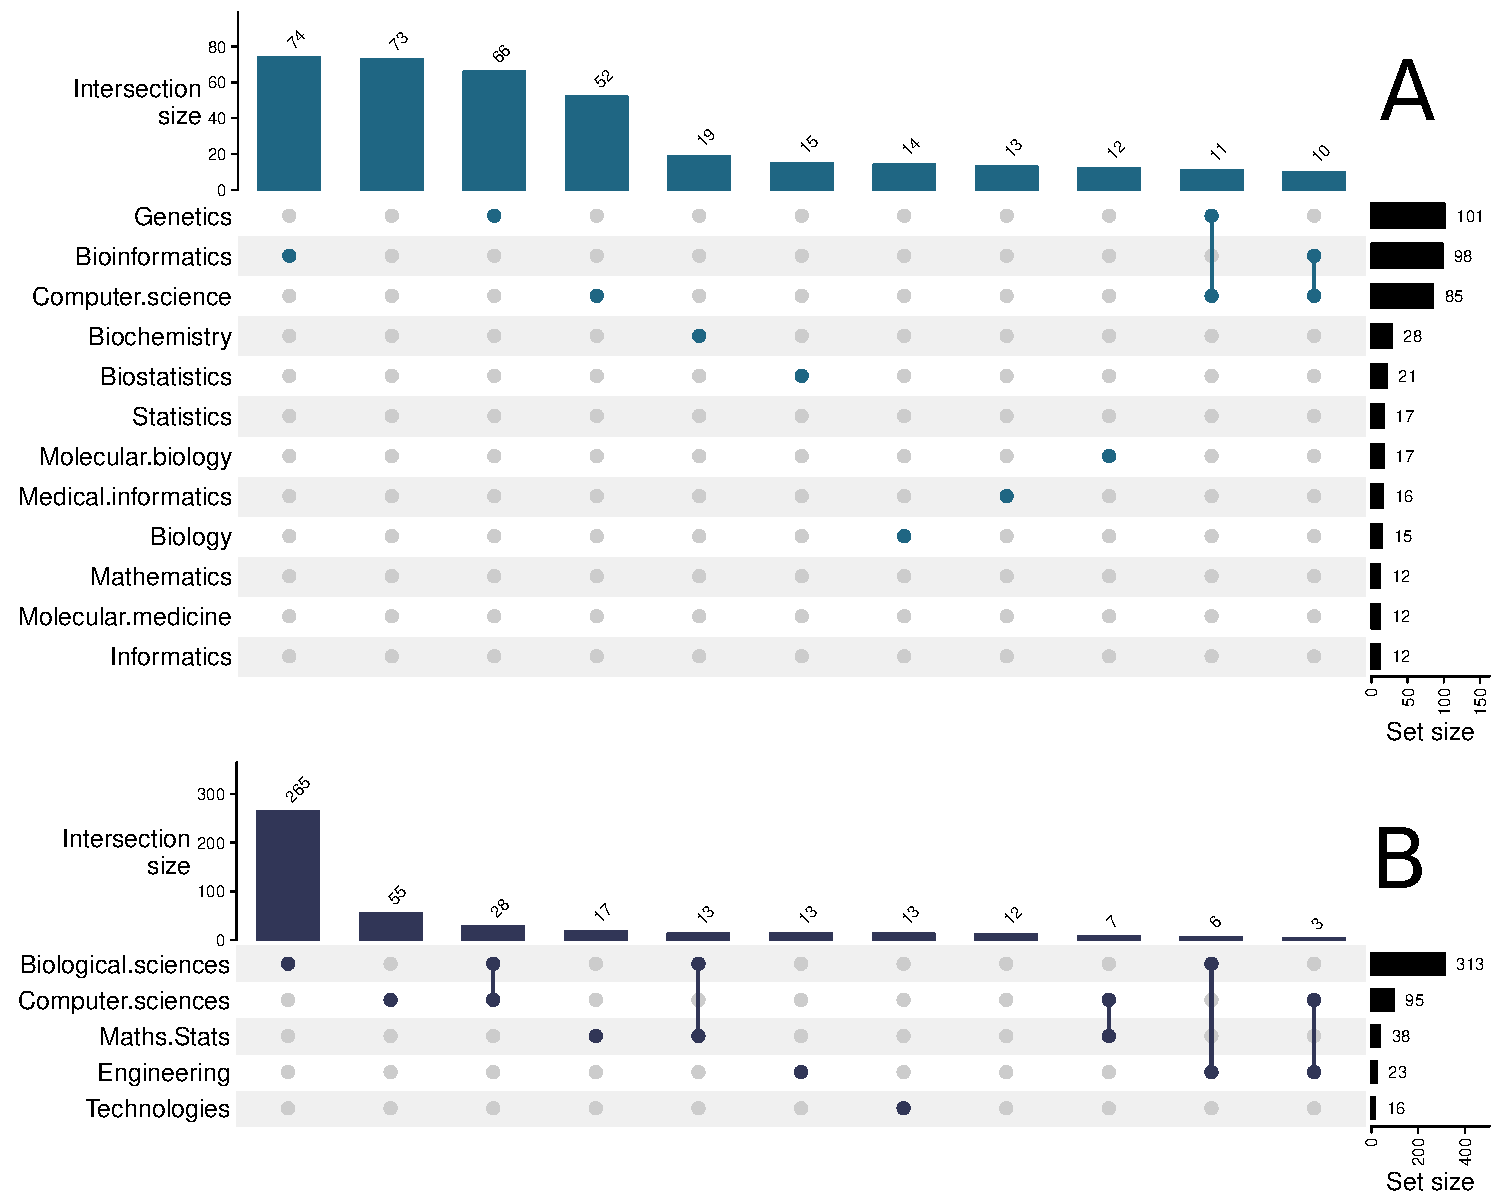
\includegraphics[width=0.6\textwidth]{upset-plots.pdf}
\end{center}
  \caption{ The number and intersection of general (\textbf{A}) or
  specific (\textbf{B}) fields that have contributed to bioinformatic
  software tools included in recent benchmark studies.  The number and
  intersection of specific fields.  }
\label{fig:fig1}
\end{figure*}


\section*{Results}

We are interested in the relationship between the accuracy of
bioinformatic software tools and academic fields of study. Using a
published corpus of accuracy rankings for bioinformatic software
tools, we have mapped software tools to academic fields and evaluated
the relationship between software accuracy and academic field.

Previously benchmarked and collated accuracy ranks were obtained from
a published supplement \cite{gardner2024}. We mapped the corresponding
author addresses for published software tools to a standardised list of
specific ``fields of study'' \cite{fields2014}, we further grouped
these into higher level general fields, and broader areas of expertise
based on the address details of each corresponding author. The number
of tools representing each general and specific field is illustrated
in Figure~\ref{fig:fig1}. The majority of bioinformatic
software is produced by corresponding authors who list at least one of
Genetics, Bioinformatics or Computer Science or similar departments as
their primary address (Figure~\ref{fig:fig1}A). For general fields, the
Biological Sciences produce the bulk of software tools, followed by
the Computer Sciences (Figure~\ref{fig:fig1}B).

\begin{figure*}[ht!]
\begin{center}
  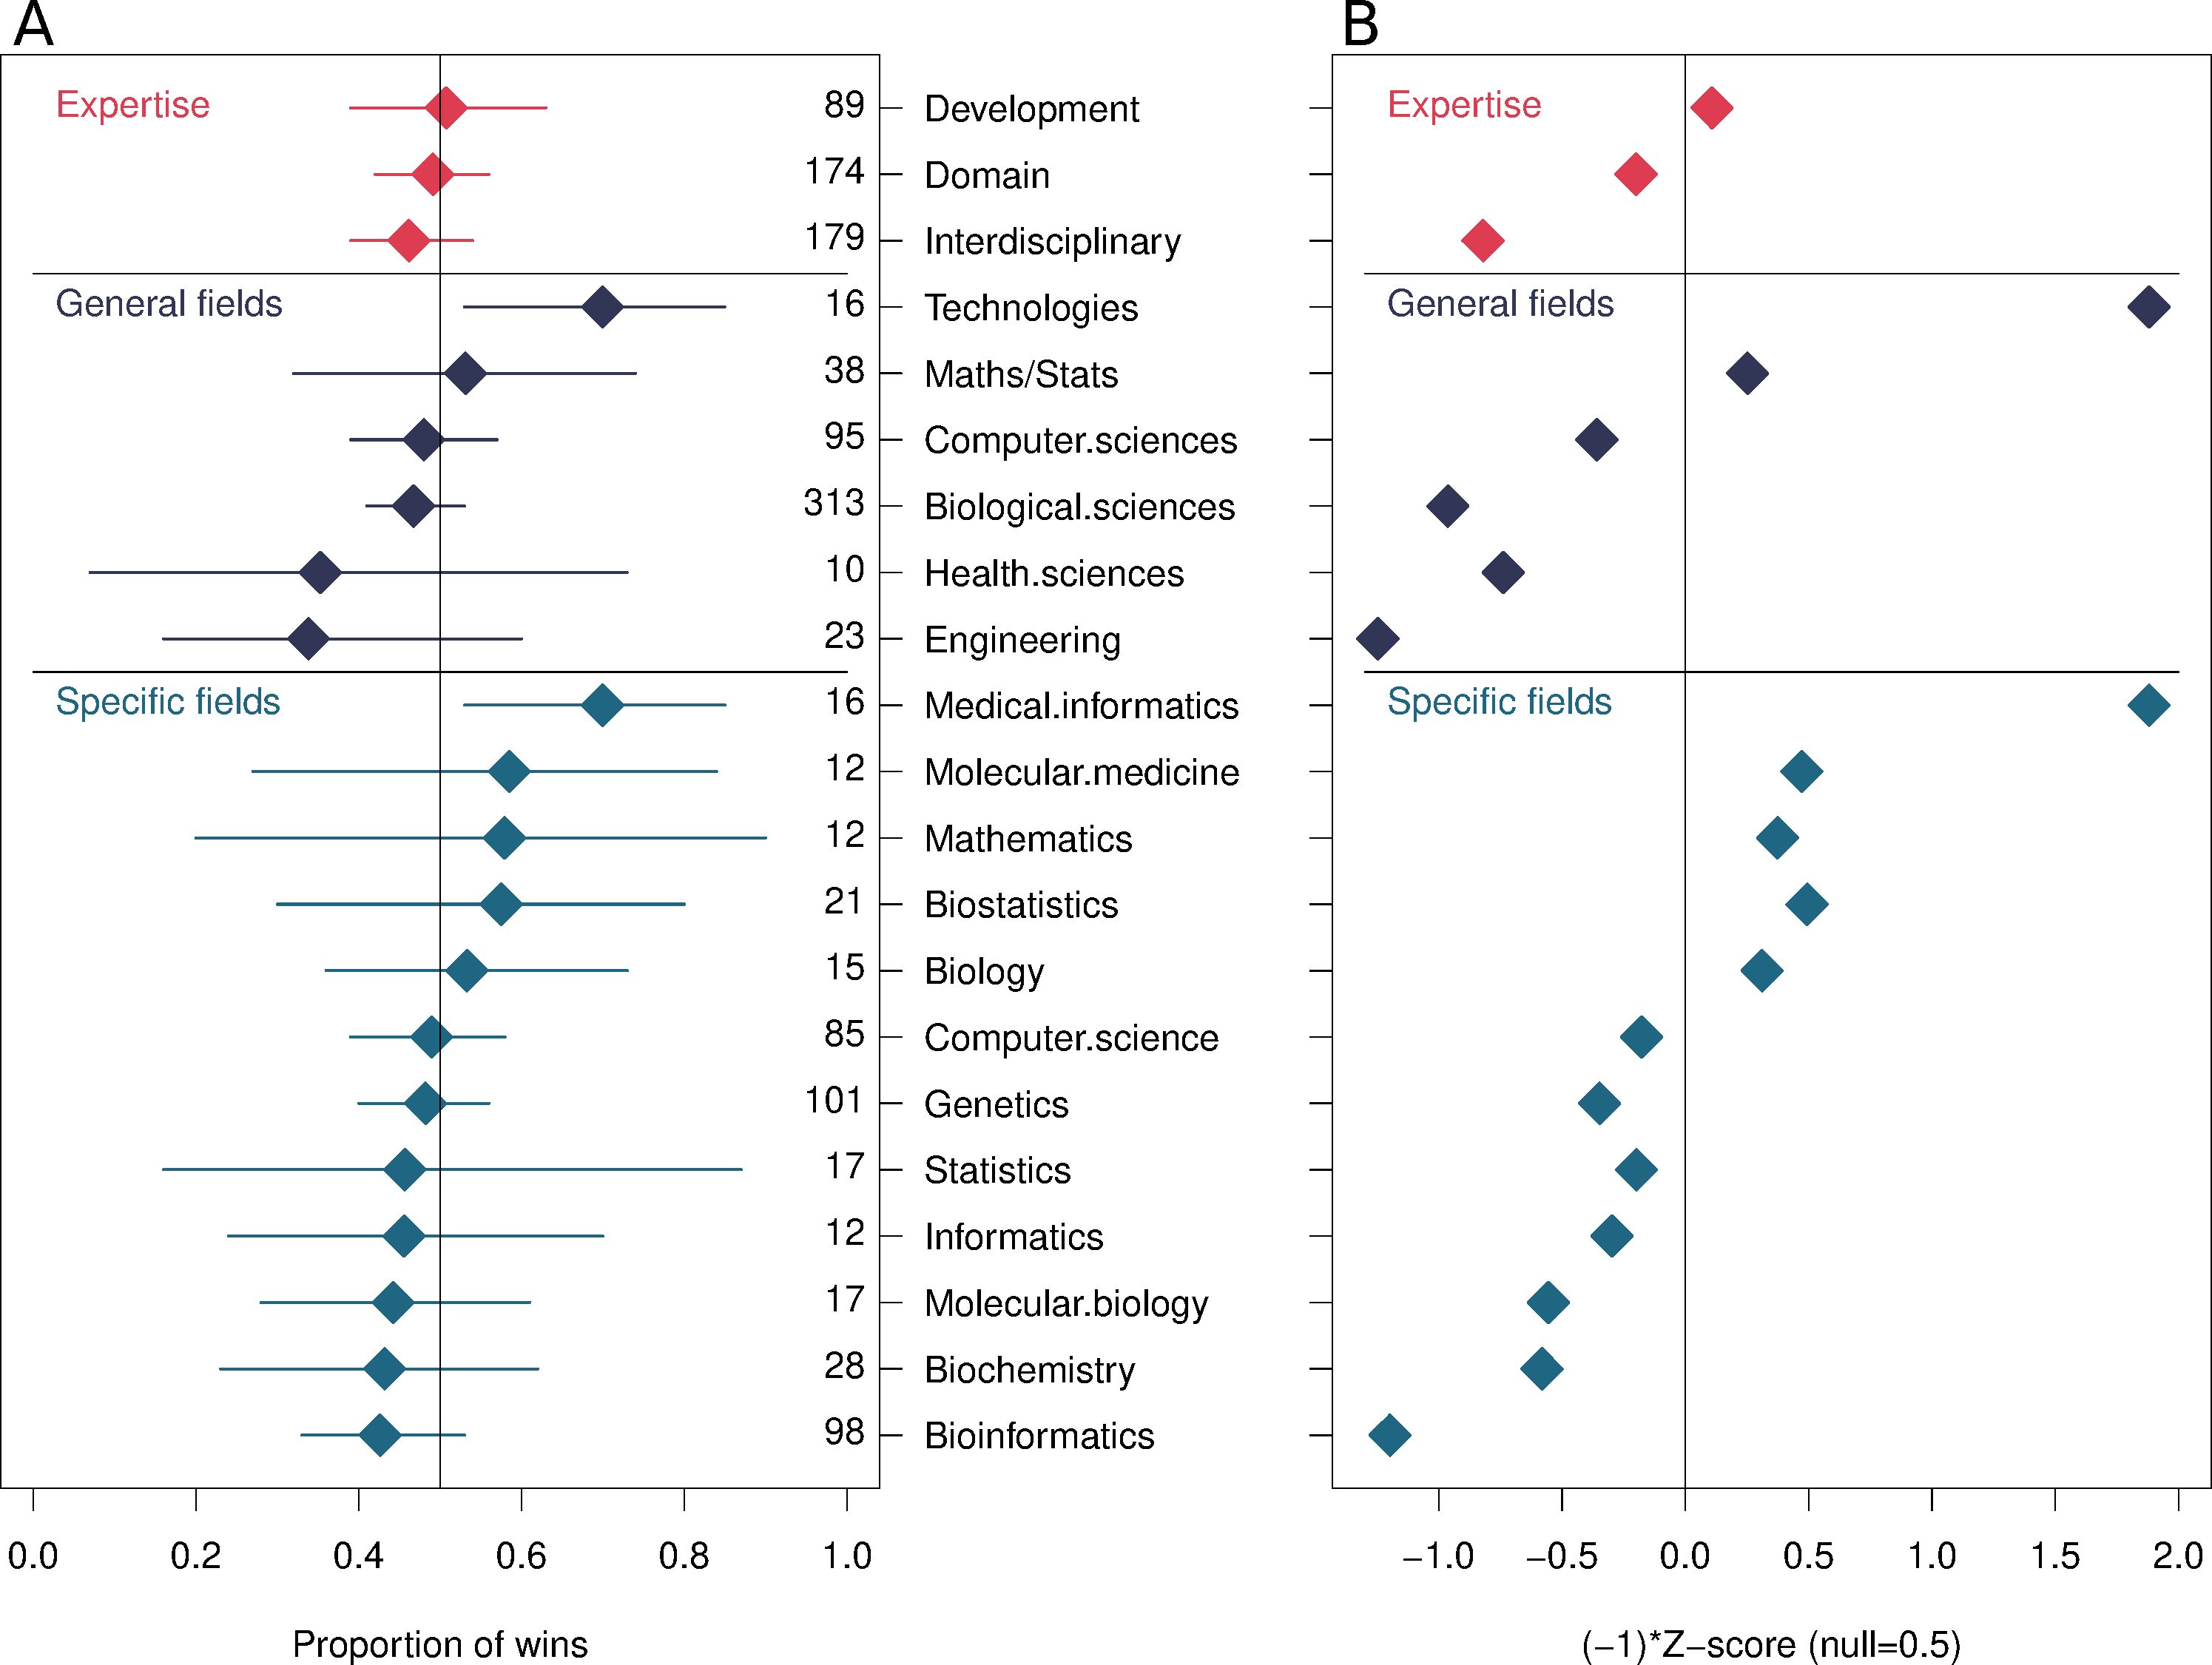
\includegraphics[width=0.8\textwidth]{forest-z-Plot.pdf}
\end{center}
\caption{(\textbf{A}) A forest plot, illustrating the mean and 95\%
  confidence intervals of the proportion of times software tools
  published by a given field ``win'' in pairwise
  comparisons. Confidence intervals and the mean was determined using
  a bootstrapping procedure. Within each field the entries have been
  sorted by the mean number of wins. The sample size for each field is
  indicated by the column of numbers on the right of the figure.
  (\textbf{B}) A Z-score was computed for each distribution of
  bootstrap samples for each field. The expected proportion of wins
  for randomly selected groups of tools was used as ``$x$''
  (i.e. null=0.5).   }
\label{fig:fig2}
\end{figure*}

The mean proportion of wins (e.g. if tool `A' outranks tool `B', this
is a win for tool `A') and the corresponding Z-scores give a way to
rank fields of study on the relative accuracy of bioinformatic
software benchmarked between 2005 and 2020 relative to the expected
number of wins for random groupings (i.e. $wins=0.5$). The greater the
proportion of wins, and $(-1)*Z-score$, then the more times tools from
a particular department outperformed competing tools in independent
benchmarks.

The specific and general fields that outperformed other
fields is ``Medical Informatics'' which is a branch of
``Technologies'', the same 16 software tools fall into both
fields. Five of which are different parameter options for the MAFFT
multiple sequence alignment tool \cite{katoh2008recent}.  These have a
mean proportion of wins of 0.70 and 95\% confidence interval of
$0.53-0.85$, which excludes the null of 0.5. The corresponding z-score
is $-1.88$ and $P=0.29$ after correcting for multiple testing.

At the other end of the spectrum is ``Bioinformatics'', ironically
authors that list ``Bioinformatics'' in their address field appear to
write less accurate software for bioinformatic
applications. The mean proportion of wins was 0.43, and 95\%
confidence interval of $0.33-0.53$. The corresponding z-score is
$1.20$ and $P=0.46$ after correcting for multiple
testing.

The general field ``Engineering'' also had a low rank. The mean
proportion of wins was just 0.34, and 95\% confidence interval of
$0.16-0.60$. The corresponding z-score is $1.25$. This general field
is made up of several smaller specific fields that includes
``Bioengineering and biomedical engineering'', ``Computer
engineering'' and ``Electrical and electronics engineering'' which
individually did not have more than ten corresponding software tools,
so were excluded from the more specific analysis.

The remaining general and specific academic fields have confidence
intervals that include the null value of 0.5, and relatively modest
z-scores that range from -0.49 to 0.96. The p-values for each were
greater than $0.05$. 

For the highest level field classifications of software development
expert, biological domain expert or interdisciplinary expert each had
similar mean proportions of wins (0.51, 0.49 and 0.46
respectively). The interdisciplinary experts had a lower z-score of
$-0.87$, which corresponds to $P=0.46$ after correcting for multiple
testing.

%followed by ``Molecular Medicine''
%We have deliberately not computed P-values or other measures of
%significance for this study. 

\section*{Conclusions and Limitations}

We have tested the assumption that the academic department subject
reflects the quality of research software. Our findings found no
significant association after multiple-testing correction between the
biological domain expert, the software developer expert or the
interdisciplinary scientist with software tool rankings on accuracy
measures. Leading us to conclude that assumptions regarding academic
department and bioinformatic software quality are likely false. The
general and specific research fields yielded similarly negative
results (Figure~\ref{fig:fig2}A).

Our earlier paper found that long-term commitments to updating
software was the leading factor associated with accurate software
tools. This current study complements that finding, showing that not
only do citation metrics (e.g. journal impact factors and author
H-index), tool age and tool speed, but also academic fields of inquiry
are \textbf{not} associated with prediction accuracy.

We focus on software tool accuracy here \cite{weber2019essential}. While speed, usability and
some features of software tools are important, in our opinion the
primary concern for bioinformatic software tools is the accuracy of
the results they produce. As poor predictions may have long-term consequences for
our general research field. 

Medical Informatics, under the broader category of "Technologies," is
identified as the top-performing group in developing accurate
bioinformatic software tools. The tools include a number of methods
for structural variation detection, single-cell profiling, long-read
assembly, multiple sequence alignment and are derived from several
different research teams. 

Bioinformatics and Engineering ranked lower in terms of software
accuracy. Tools developed by authors who affiliated with
"Bioinformatics" typically had slightly lower accuracy than that of
other fields. However, this was not a statistically significant
finding. In addition (further bad news for this author),
``Biochemistry'' was similarly ranked, again this was not a
statistically significant finding.

This leads us to conclude that an individual's host department are not
reflective of the quality of software that they are capable of
producing ($p>0.05$ in all instances). As a consequence, the academic
department should not be used as a proxy for judging the potential of
software development projects.

%Limitations mentioned in the conclusion could be expanded to better discuss how they may affect the study's findings and their implications.

This study has several limitations. Some benchmarks rank several tool
options, the effects of which may be modest to large, and potentially
non-independent. The number of accuracy metrics used is also diverse,
some of which may be flawed in some circumstances. For example,
``accuracy'' with large class-imbalance \cite{luque2019impact}, or N50
which some commentators have criticised \cite{xie2021pdr}. Some
benchmarks are relatively small resulting in small changes in rank
having a potentially large impact on the proportion of wins. Finally,
the cohort of benchmarks has not been updated to include more recent
results.

There is likely a disconnect between training and the host department
for many bioinformatic tool developers. For example, this author
studied mathematics as an undergraduate, conducted a PhD in
bioinformatics, held postdoctoral fellowships in computer science and
molecular biology departments, spent several years at a genomics
research institute and is now employed in a Biochemistry
Department. The ``Biochemistry'' departmental label is not an accurate
reflection of my training or recent publications. I certainly can't
recall any of the key steps of glycolysis, the citric acid cycle or
the structure of any amino acid or protein.

The last, corresponding author is generally the principal investigator
leading a project. They may have limited involvement in the actual
development of any software tool while they (supposedly) provide
resources for the project and overall direction. However, there is a
significant overlap between the department of a first author, who
would generally be the primary developer of a tool, and the last
author (not tested here). Therefore we expect these results to be
broadly similar if first-author departments were used instead. 

%OPen questions: what impact does training have on improving software quality?
%                

%We end with echoing the call for more training and a continued 
%\cite{johanson2018software,siepel2019challenges}

\section*{Methods}

~~~~\textbf{Pre-registration:} This study's desired sample size, included variables, hypotheses, and
planned analyses were pre-registered on the Open Science Framework
%(https://doi.org/10.17605/OSF.IO/92PTZ)
prior to any unpublished data being collected \cite{gardner2024}.

\textbf{Benchmarking data:} software ranks from previously gathered
benchmarks are publically available \cite{Gardner:2022}, these include data from
68 publications that rank the accuracy of different sets of 498
distinct software tools.

%The methodology section should provide more detail about how the software tools were selected and mapped to academic fields. It’s important to describe how biases or inconsistencies in mapping were addressed.
\textbf{Mapping tools to academic field:} For each software tool, when
available, the corresponding publication(s) were identified and the
addresses for the primary corresponding author were extracted
manually. In cases where an author lists multiple addresses, just the
first two are used. When multiple corresponding authors were listed,
the last corresponding author was selected.

The author department names were mapped to the closest associated
``fields of study'' listed by the National Science Foundation
\cite{fields2014}. We analysed fields at three different hierarchical
levels, firstly the specific fields (e.g. ``genetics'', ``computer
science'', ``bioinformatics'' etc). These are then mapped to more
general fields within the ``fields of study'' classification
(e.g. ``biological sciences'', ``computer sciences'' etc). We have
further mapped these to three expertise types, the \textbf{development
  experts}, \textbf{domain experts} and \textbf{interdisciplinary
  experts}. The development experts are from fields such as computer
science, mathematics and engineering, they are expected to bring
development-pertinent expertise in software engineering and
mathematical modeling of biological problems. The domain experts are
drawn from the biological and health sciences and are expected to have
detailed knowledge of the subject area and be invested in producing
high-performing software for their research. The interdisciplinary
experts are drawn from interdisciplinary subjects such as
bioinformatics, biostatistics and biomathematics. Additionally the
researchers who list both development and domain expertise in their
addresses (e.g. ``Computer Science'' and ``Genetics''). We have treated some fields as essentially synonymous, for
example departments of ``Computational Biology'' was mapped to
``Bioinformatics'', and ``Genomics'' is mapped to ``Genetics''.

We restricted all subsequent analyses to fields that contain at least 10
software tools in our benchmark corpus. This mitigated against
potential issues due to small sample sizes. 

\textbf{Statistical analysis:} The accuracy data is derived from
benchmarks using a diverse number of metrics that include sensitivity,
specificity, PPV, FDR, error rates, AUROC, MCC and others
\cite{weber2019essential}. The number of tools ranked in any benchmark
ranged from 3 to 50. In order to obtain a representative measure of
accuracy for a field that transcends diverse accuracy measures and
numbers of ranked tools we elected to use ranks and a
bootstrapping strategy.  We randomly sample with replacement sets of
200 tools (from the total of 498), a benchmark that includes each tool
is selected at random and the number of times the tool ``won'' against
another tool is recorded, as is the total number of pairwise
comparisons that were made. These counts of wins and total comparisons
are transferred to the corresponding specific, general and expertise
areas. This is repeated 1,000 times, and allows a way to estimate the
mean proportions of wins allocated to each field, and a 95\%
confidence interval for this value (Figure~\ref{fig:fig2}A). We also compute a
Z-score for each field using the below equation. This measures the
number of standard deviations the mean number of wins is from the
expected null value of 0.5 for randomly grouped tools
(Figure~\ref{fig:fig2}B).

$z=\frac{x-\mu}{\sigma}$


%\textbf{WRITE UP: Bootstrapping, mean number of wins, confidence intervals, forest plot. }


Where $\mu$ is the mean, $\sigma$ is the standard deviation, $x$ is the raw
value. In this case we set $x=0.5$ as this is the null expectation for
the proportion of wins for randomly grouped sets of tools. For the
purposes of illustration we plot $(-1)*z$ so that the direction is the
same as for the ``proportion of wins'' forest plot
(Figure~\ref{fig:fig1}). 

P-values are computed from the absolute value of the z-scores to
evaluate if any field is significantly distinguished from the null
i.e. $P[X > x]$. The P-values are corrected for multiple testing by
controlling the false discovery rate method
\cite{benjamini1995controlling}.


\noindent\textbf{Data and analysis scripts availability}

The data, scripts, figures and manuscript draft files are availble at the GitHub repository:\\
\href{https://github.com/ppgardne/departments-software-accuracy}{https://github.com/ppgardne/departments-software-accuracy}

\noindent\textbf{Funding:} This research was supported by the MBIE data
science platform ``Beyond Prediction: explanatory and transparent data
science'', Genomics Aotearoa, and Marsden
Grants 19-UOO-040 and 20-UOA-282.

\noindent\textbf{Authors' contributions:} this work was conceived by 
PPG, designed by PPG, the analysis was carried out by PPG, interpretation of the results was by PPG,
the manuscript was drafted by  PPG.
All authors revised and edited the final manuscript. All authors approve the submitted version. 

%----------------------------------------------------------------------------------------
%       REFERENCE LIST
%----------------------------------------------------------------------------------------
\bibliographystyle{unsrt}
\bibliography{references.bib}


\end{document}
